\section{Experiments}

\subsection{Simulating MPC}

\begin{figure}[H]
\centering
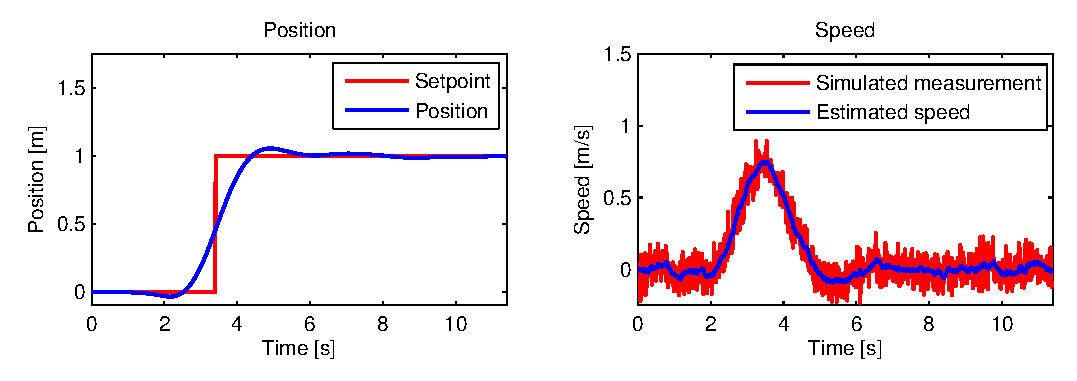
\includegraphics[width=0.99\textwidth]{fig/simulation1_step_no_governor.eps}
\caption{Simulating position step response without the input governor.}
\label{fig:simulation_step_no_governor}
\end{figure}

\begin{figure}[H]
\centering
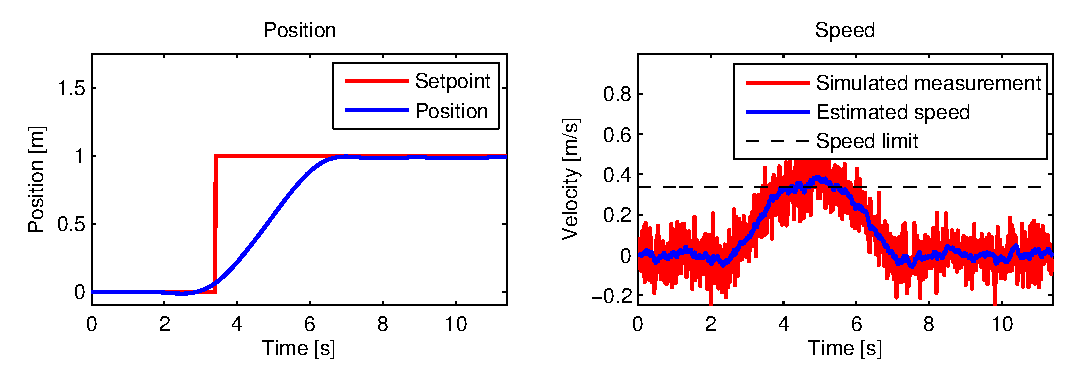
\includegraphics[width=0.99\textwidth]{fig/simulation2_step_governor.eps}
\caption{Simulating position step response with the input governor.}
\label{fig:simulation_step_governor}
\end{figure}

\begin{figure}[H]
\centering
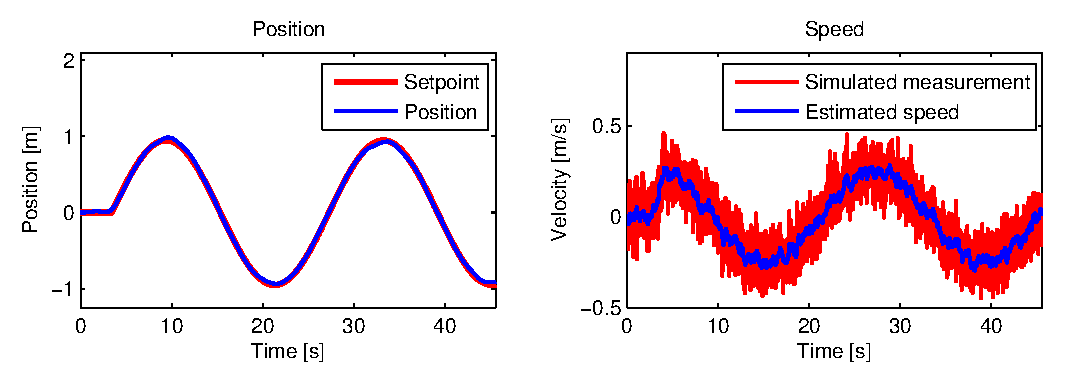
\includegraphics[width=0.99\textwidth]{fig/simulation3_sine.eps}
\caption{Simulating trajectory of feasible sine trajectory.}
\label{fig:simulation_step_governor}
\end{figure}

\begin{figure}[H]
\centering
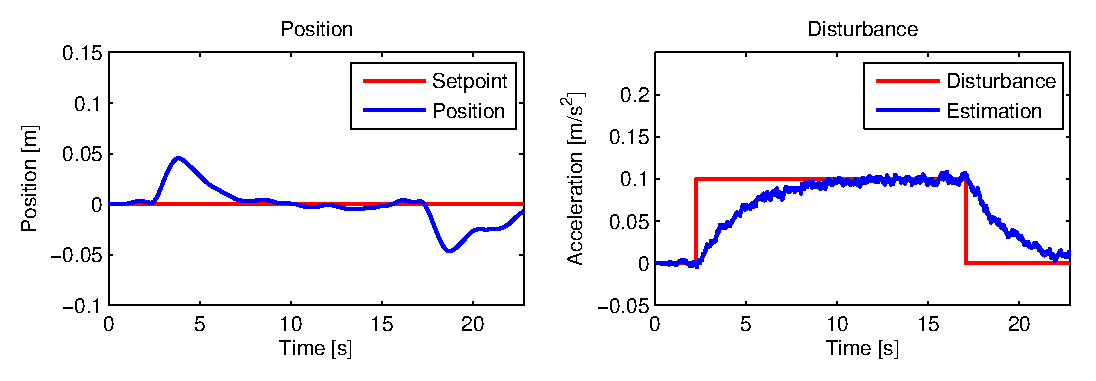
\includegraphics[width=0.99\textwidth]{fig/simulation4_disturbance_rejection.eps}
\caption{Simulating of disturbance rejection.}
\label{fig:simulation_step_governor}
\end{figure}

\subsection{Tracking constant setpoint \& position drift}

\begin{figure}[H]
\centering
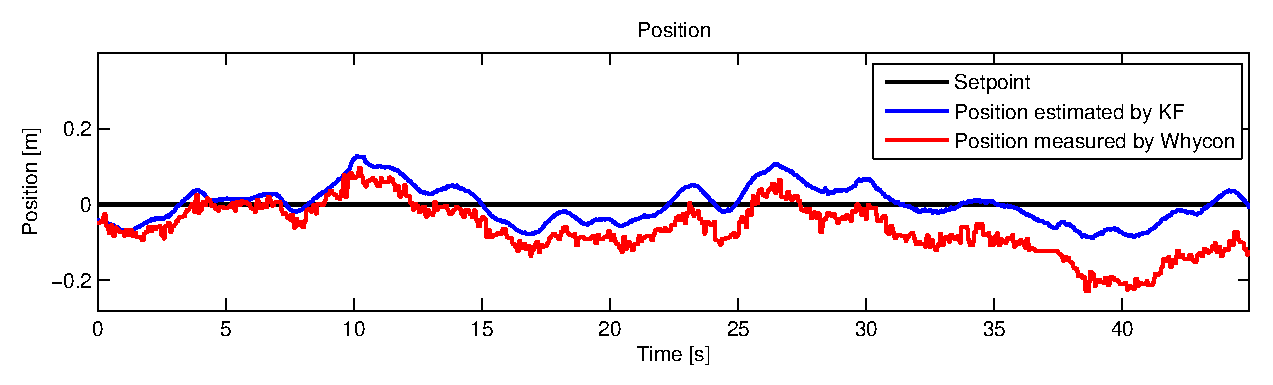
\includegraphics[width=0.99\textwidth]{fig/experiment5_drift_constant.eps}
\caption{Experiment with tracking static trajectory.}
\label{fig:experiment_sine_1}
\end{figure}

\subsection{Tracking dynamic trajectory}
\label{cap:dynamic_trajectory_tracking}

\begin{figure}[h]
\centering
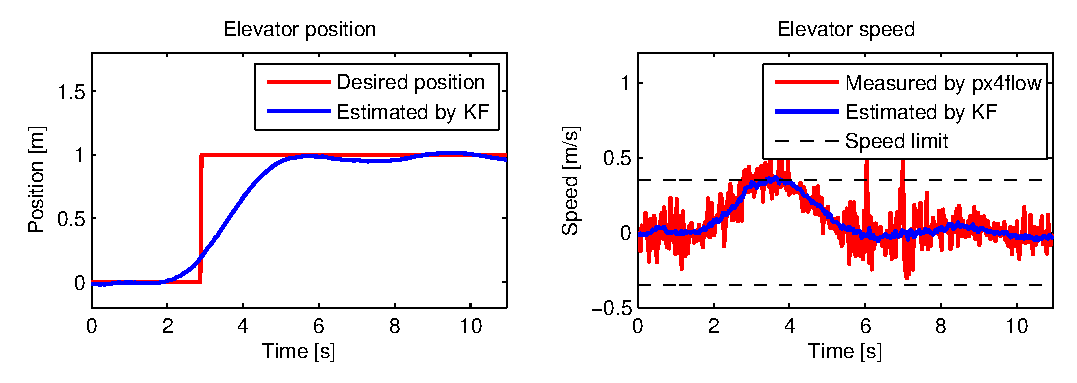
\includegraphics[width=0.99\textwidth]{fig/experiment2_step.eps}
\caption{Experiment with step response.}
\label{fig:experiment_sine_1}
\end{figure}

\begin{figure}[H]
\centering
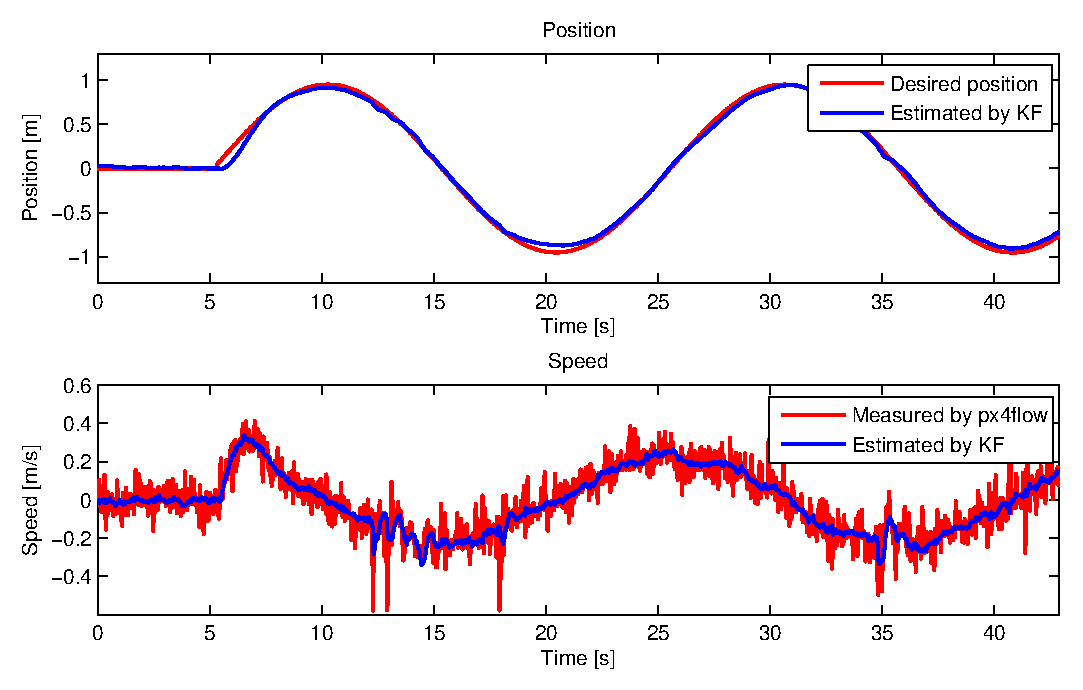
\includegraphics[width=0.99\textwidth]{fig/experiment1_sine.eps}
\caption{Experiment with tracking circular trajectory. Figures show position and velocity in single axis. Amplitude $0.95\jed{m}$, period $20\jed{s}$.}
\label{fig:experiment_sine_1}
\end{figure}

\begin{figure}[H]
\centering
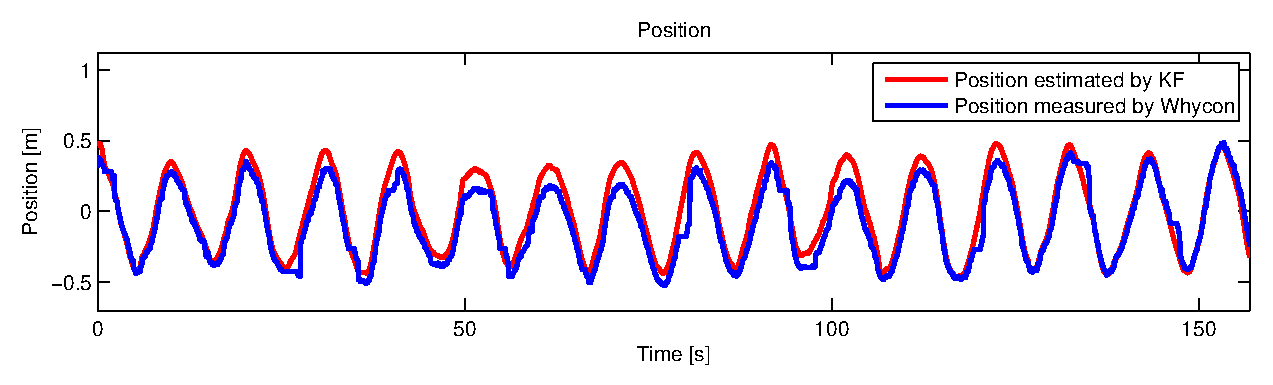
\includegraphics[width=0.99\textwidth]{fig/experiment5_drift_sine.eps}
\caption{Experiment with tracking sine trajectory.}
\label{fig:experiment_drift_sine}
\end{figure}

\subsection{Disturbance rejection}

\subsubsection{Persistent wind disturbances}

\begin{figure}[H]
\centering
	\begin{tikzpicture}
		\node[anchor=south west,inner sep=0] (a) at (0,0) {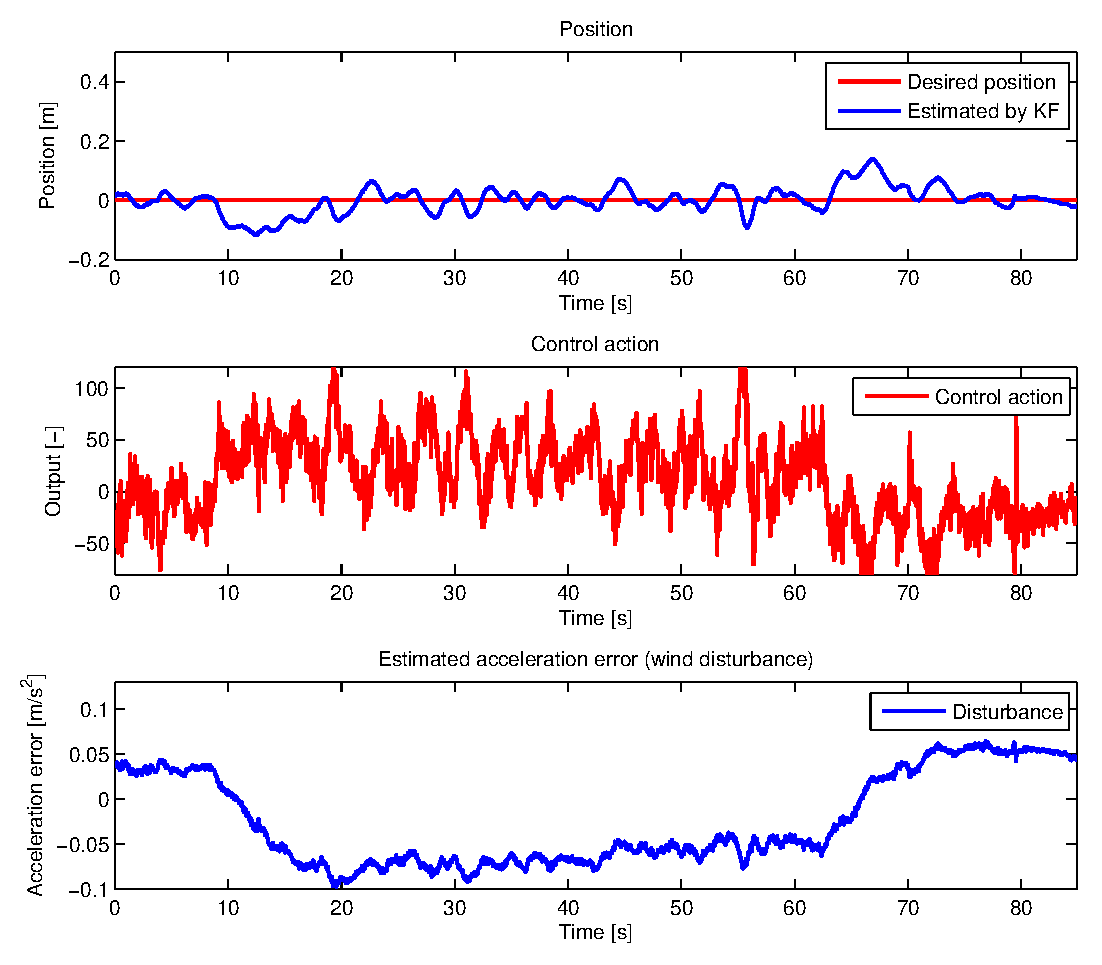
\includegraphics[width=\textwidth]{fig/experiment3_steady_disturbance.eps}};
		\begin{scope}[x={(a.south east)},y={(a.north west)}]

		%\draw[help lines,xstep=.1,ystep=.1] (0,0) grid (1,1);	
		
%        \draw[white,ultra thick,rounded corners] (0.55,0.50) rectangle (0.7,0.7);
%        \draw (0.58,0.655) node [text=white] {\textbf{1}};
        

		%\draw[-latex] (0.2,0.9) -- (0.2,0.81);    
		%\node[] at (0.25,0.92) {Disturbance started};    
		
		%\draw[-latex] (0.75,0.9) -- (0.795,0.81);    
		%\node[] at (0.65,0.92) {Disturbance went off};  
		
		\draw[fill=gray, opacity=0.2] (0.2,0.740) rectangle (0.757,0.960);  
		
		\draw[fill=gray, opacity=0.2] (0.2,0.401) rectangle (0.757,0.625);  
		
		\draw[fill=gray, opacity=0.2] (0.2,0.064) rectangle (0.757,0.287);  
        
    \end{scope}
	\end{tikzpicture}
\caption{Experiment with tracking constant setpoint while being under the influence of wind.}
\label{fig:experiment_steady_wind}
\end{figure}

\subsubsection{Momentary disturbances}
\label{cap:momentary_disturbances}

\begin{figure}[H]
\centering
	\begin{tikzpicture}
		\node[anchor=south west,inner sep=0] (a) at (0,0) {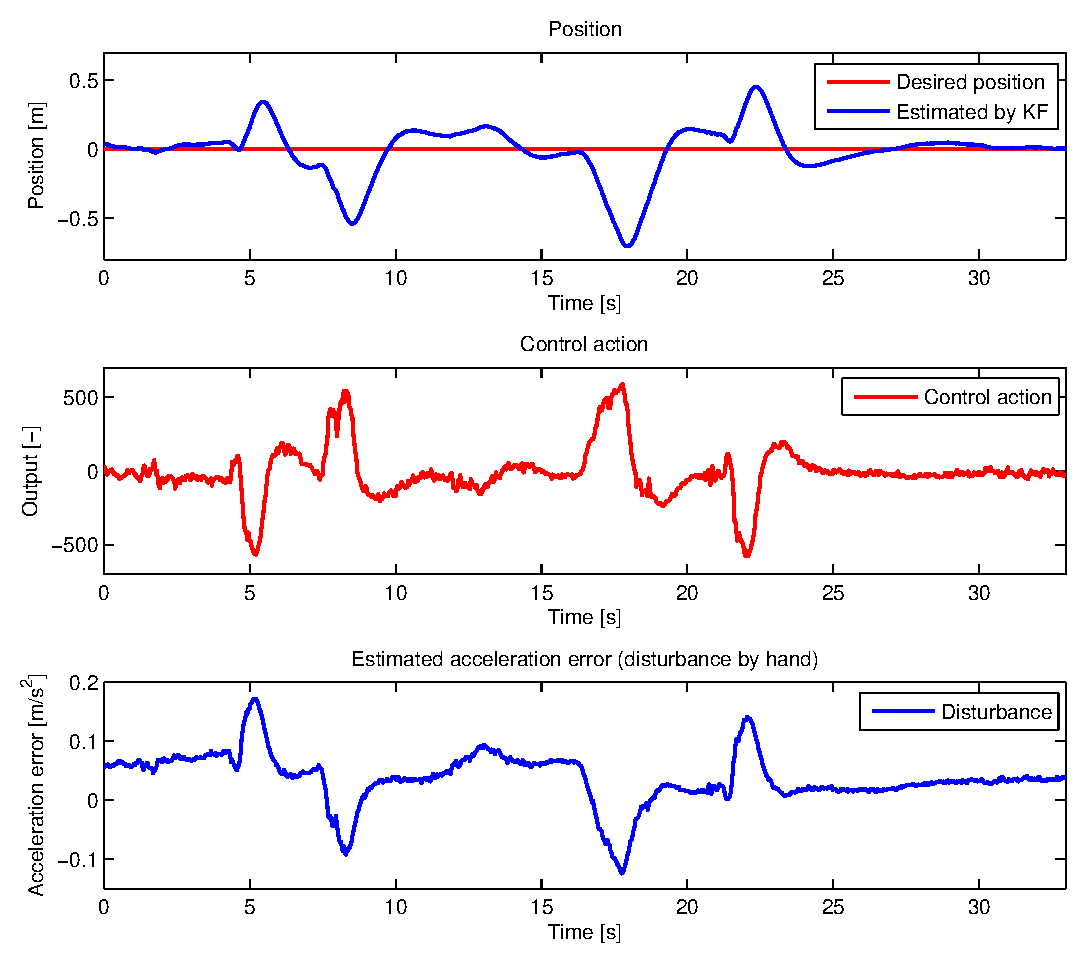
\includegraphics[width=\textwidth]{fig/experiment4_sudden_disturbances.eps}};
		\begin{scope}[x={(a.south east)},y={(a.north west)}]

		%\draw[help lines,xstep=.1,ystep=.1] (0,0) grid (1,1);	
		
%        \draw[white,ultra thick,rounded corners] (0.55,0.50) rectangle (0.7,0.7);
%        \draw (0.58,0.655) node [text=white] {\textbf{1}};
        

		\draw[fill=gray, opacity=0.2] (0.205,0.739) rectangle (0.235,0.960);  
		\draw[fill=gray, opacity=0.2] (0.29,0.739) rectangle (0.319,0.96);  
		\draw[fill=gray, opacity=0.2] (0.41,0.739) rectangle (0.445,0.96);  
		\draw[fill=gray, opacity=0.2] (0.532,0.739) rectangle (0.575,0.96);  
		\draw[fill=gray, opacity=0.2] (0.675,0.739) rectangle (0.7,0.96); 
		
		\draw[fill=gray, opacity=0.2] (0.205,0.400) rectangle (0.235,0.625);  
		\draw[fill=gray, opacity=0.2] (0.29,0.400) rectangle (0.319,0.625);  
		\draw[fill=gray, opacity=0.2] (0.41,0.400) rectangle (0.445,0.625);  
		\draw[fill=gray, opacity=0.2] (0.532,0.400) rectangle (0.575,0.625);  
		\draw[fill=gray, opacity=0.2] (0.675,0.400) rectangle (0.7,0.625); 
		
		\draw[fill=gray, opacity=0.2] (0.205,0.064) rectangle (0.235,0.286);  
		\draw[fill=gray, opacity=0.2] (0.29,0.064) rectangle (0.319,0.286);  
		\draw[fill=gray, opacity=0.2] (0.41,0.064) rectangle (0.445,0.286);  
		\draw[fill=gray, opacity=0.2] (0.532,0.064) rectangle (0.575,0.286);  
		\draw[fill=gray, opacity=0.2] (0.675,0.064) rectangle (0.7,0.286); 
        
    \end{scope}
	\end{tikzpicture}
\caption{Experiment with tracking constant setpoint while being under the influence of momentary disturbances. The UAV was dragged by hand.}
\label{fig:experiment_steady_wind}
\end{figure}

\subsection{Summary and comparison with previous work}